\subsection{Motivation for optimisation approach}
Most approaches to designing Bézier polynomial-based virtual constraints for a bipedal robot can be classed in one of three categories; \textit{manual design}, \textit{sampling} and \textit{optimisation}. Manual design involves a human operator producing the control points directly. Sampling is the utilisation of some method of choosing coefficients in an attempt to span the configuration space, either by random selection or gridding. Optimisation approaches choose coefficients which minimise some cost function under particular constraints.

Manual design approaches are not favourable since they are expensive and very slow in comparison to automatic generation of constraints. Sampling methods, while much faster at generating a single constraint than manual generation, suffer from the \textit{curse of dimensionality}. That is, in order for a sampling method to produce the same density of coverage, the number of samples required increases exponentially with the number of dimensions.

Under most definitions, the optimality of a planned trajectory cannot exceed the optimality of the primitives which compose it.

\subsection{Definition of optimality}
As with most physical systems, there is a lack of consensus in the definition of optimality in the case walking robots; {\color{red}<insert literature references to competing definitions>}.

The definition of optimality chosen for the purposes of producing the virtual constraint library is as follows:

\emph{The optimal constraint for a given start and end configuration and kinetic energy gain or loss is the one which requires the minimum energy input to maintain.}

We note that the relationship between torque and electrical energy in conventional DC motors is typically approximated by the following equation: \cite{??}
\begin{equation}
	E = \int\limits_0^t u^2 ds
\end{equation}

Using this definition, we may further motivate the need for optimisation of the virtual constraints by way of example. Consider Figure \ref{fig:manualgen}; the constraint has been chosen based upon reasoning that it appears to produce a net-gain kinetic energy in a fairly smooth motion. However, the torque required to maintain this motion is clearly wasteful and nonmonotonic. {\color{red} Maybe try to give some good justification here.}

\begin{figure}
	\centering
	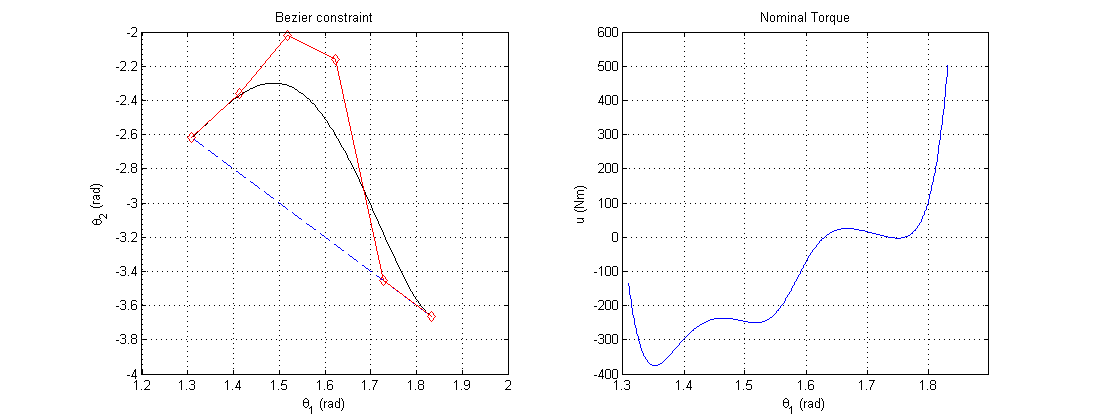
\includegraphics[width=0.9\linewidth]{4VirtConstLib/manualgen.png}
	\caption{Torque curve for manually generated constraint}
	\label{fig:manualgen}
\end{figure}

\subsection{Validity of convex optimisation approach}
{\color{blue} Note on intractability of gridding approaches}
Surfaces which confirm quasi-convexity.

\subsection{Optimisation method}
Unfortunately, the torque required to maintain a constraint varies with initial velocity. Since the virtual constraint library is prepared off-line, the initial velocity is unknown. The constraint is therefore optimised over a nominal trajectory. That is, each virtual constraint is only perfectly optimised for a particular initial velocity. {\color{red} Justify this, and go into depth about the choice of initial velocity? There's no reason that this should be the same per constraint. The nominal trajectory is probably different for each constraint.}

The nominal initial velocity for a particular constraint was chosen to be that which achieves periodic walking based upon the constraint. That is, the output of the impact map $\dot{\theta}^+$ is equal to the initial velocity $\dot{\theta}_0$. This is calculable in closed-form (with $\Delta_{\dot{\theta}}$ as defined in Equation \ref{eqn:Delthd}):
\begin{subequations}
\begin{align}
	\left(\dot{\theta}^-\right)^2 &= \Gamma(\theta^-)\dot{\theta}_0^2 + \Psi(\theta^-) \\
	\dot{\theta}^+ &= c\Delta_{\dot{\theta}}\dot{\theta}^-
\end{align}
\end{subequations}
Equating $\dot{\theta}^+$ and $\dot{\theta}_0$, we obtain (periodic velocity)
\begin{equation}
	\dot{\theta}_{0,p}^2 = \frac{\Psi(\theta^-)}{(c\Delta_{\dot{\theta}})^{-2} - \Gamma(\theta^-)}
\end{equation}
Achieving fixed post-impact velocity:
\begin{equation}
	\dot{\theta}_{0,f}^2 = \frac{(c\Delta_{\dot{\theta}})^{-2}\dot{\theta}_f^2 - \Psi(\theta^-)} {\Gamma(\theta^-)}
\end{equation}
Equating $\dot{\theta}^+$ with $\lambda\dot{\theta}_{0,c}$ (Achieving fixed ratio $\lambda$ over minimum velocity to complete footstep):
\begin{equation}
	\dot{\theta}_{0,\lambda}^2 = \frac{(c\Delta_{\dot{\theta}})^{-2}\left(-\lambda^2\frac{ \Psi(\theta_c)}{ \Gamma(\theta_c)}\right) - \Psi(\theta^-)} {\Gamma(\theta^-)}
\end{equation}
{\color{blue} Why do this instead of just using $\dot{\theta}_0 = \lambda\dot{\theta}_{0,c}$? I think it's better because it takes into account the impacts and therefore more realistically defines the required velocity for the constraint. I need to think this through a bit more. Maybe in this section go through all of the logical alternatives to setting up the nominal velocity and justify which is best.}

{\color{red} Also need to include constraints - friction cone and invariance. Note choice of zero slope to allow for velocity invariance to be satisfied and friction cone being dependent only on the configuration, since the forces themselves are dependent on the velocity, but the ratio is fixed by the constraint; $F_2$ is linear in $\dot{q}$. Also, perhaps discuss using time basis/using theta basis; theta basis may be skewed since it is not linear in time, so integral of torque as a function of theta gives a different result to integral of torque as a function of time. We can derive time-based torque at the cost of additional computation}